\documentclass[twoside]{book}

% Packages required by doxygen
\usepackage{fixltx2e}
\usepackage{calc}
\usepackage{doxygen}
\usepackage[export]{adjustbox} % also loads graphicx
\usepackage{graphicx}
\usepackage[utf8]{inputenc}
\usepackage{makeidx}
\usepackage{multicol}
\usepackage{multirow}
\PassOptionsToPackage{warn}{textcomp}
\usepackage{textcomp}
\usepackage[nointegrals]{wasysym}
\usepackage[table]{xcolor}

% Font selection
\usepackage[T1]{fontenc}
\usepackage[scaled=.90]{helvet}
\usepackage{courier}
\usepackage{amssymb}
\usepackage{sectsty}
\renewcommand{\familydefault}{\sfdefault}
\allsectionsfont{%
  \fontseries{bc}\selectfont%
  \color{darkgray}%
}
\renewcommand{\DoxyLabelFont}{%
  \fontseries{bc}\selectfont%
  \color{darkgray}%
}
\newcommand{\+}{\discretionary{\mbox{\scriptsize$\hookleftarrow$}}{}{}}

% Page & text layout
\usepackage{geometry}
\geometry{%
  a4paper,%
  top=2.5cm,%
  bottom=2.5cm,%
  left=2.5cm,%
  right=2.5cm%
}
\tolerance=750
\hfuzz=15pt
\hbadness=750
\setlength{\emergencystretch}{15pt}
\setlength{\parindent}{0cm}
\setlength{\parskip}{3ex plus 2ex minus 2ex}
\makeatletter
\renewcommand{\paragraph}{%
  \@startsection{paragraph}{4}{0ex}{-1.0ex}{1.0ex}{%
    \normalfont\normalsize\bfseries\SS@parafont%
  }%
}
\renewcommand{\subparagraph}{%
  \@startsection{subparagraph}{5}{0ex}{-1.0ex}{1.0ex}{%
    \normalfont\normalsize\bfseries\SS@subparafont%
  }%
}
\makeatother

% Headers & footers
\usepackage{fancyhdr}
\pagestyle{fancyplain}
\fancyhead[LE]{\fancyplain{}{\bfseries\thepage}}
\fancyhead[CE]{\fancyplain{}{}}
\fancyhead[RE]{\fancyplain{}{\bfseries\leftmark}}
\fancyhead[LO]{\fancyplain{}{\bfseries\rightmark}}
\fancyhead[CO]{\fancyplain{}{}}
\fancyhead[RO]{\fancyplain{}{\bfseries\thepage}}
\fancyfoot[LE]{\fancyplain{}{}}
\fancyfoot[CE]{\fancyplain{}{}}
\fancyfoot[RE]{\fancyplain{}{\bfseries\scriptsize Generated by Doxygen }}
\fancyfoot[LO]{\fancyplain{}{\bfseries\scriptsize Generated by Doxygen }}
\fancyfoot[CO]{\fancyplain{}{}}
\fancyfoot[RO]{\fancyplain{}{}}
\renewcommand{\footrulewidth}{0.4pt}
\renewcommand{\chaptermark}[1]{%
  \markboth{#1}{}%
}
\renewcommand{\sectionmark}[1]{%
  \markright{\thesection\ #1}%
}

% Indices & bibliography
\usepackage{natbib}
\usepackage[titles]{tocloft}
\setcounter{tocdepth}{3}
\setcounter{secnumdepth}{5}
\makeindex

% Hyperlinks (required, but should be loaded last)
\usepackage{ifpdf}
\ifpdf
  \usepackage[pdftex,pagebackref=true]{hyperref}
\else
  \usepackage[ps2pdf,pagebackref=true]{hyperref}
\fi
\hypersetup{%
  colorlinks=true,%
  linkcolor=blue,%
  citecolor=blue,%
  unicode%
}

% Custom commands
\newcommand{\clearemptydoublepage}{%
  \newpage{\pagestyle{empty}\cleardoublepage}%
}

\usepackage{caption}
\captionsetup{labelsep=space,justification=centering,font={bf},singlelinecheck=off,skip=4pt,position=top}

%===== C O N T E N T S =====

\begin{document}

% Titlepage & ToC
\hypersetup{pageanchor=false,
             bookmarksnumbered=true,
             pdfencoding=unicode
            }
\pagenumbering{roman}
\begin{titlepage}
\vspace*{7cm}
\begin{center}%
{\Large My Project }\\
\vspace*{1cm}
{\large Generated by Doxygen 1.8.11}\\
\end{center}
\end{titlepage}
\clearemptydoublepage
\tableofcontents
\clearemptydoublepage
\pagenumbering{arabic}
\hypersetup{pageanchor=true}

%--- Begin generated contents ---
\chapter{File Index}
\section{File List}
Here is a list of all files with brief descriptions\+:\begin{DoxyCompactList}
\item\contentsline{section}{\hyperlink{Lab1_8c}{Lab1.\+c} }{\pageref{Lab1_8c}}{}
\end{DoxyCompactList}

\chapter{File Documentation}
\hypertarget{Lab1_8c}{}\section{Lab1.\+c File Reference}
\label{Lab1_8c}\index{Lab1.\+c@{Lab1.\+c}}
{\ttfamily \#include $<$stdio.\+h$>$}\\*
{\ttfamily \#include $<$string.\+h$>$}\\*
{\ttfamily \#include $<$sys/types.\+h$>$}\\*
{\ttfamily \#include $<$fcntl.\+h$>$}\\*
{\ttfamily \#include $<$unistd.\+h$>$}\\*
Include dependency graph for Lab1.\+c\+:
\nopagebreak
\begin{figure}[H]
\begin{center}
\leavevmode
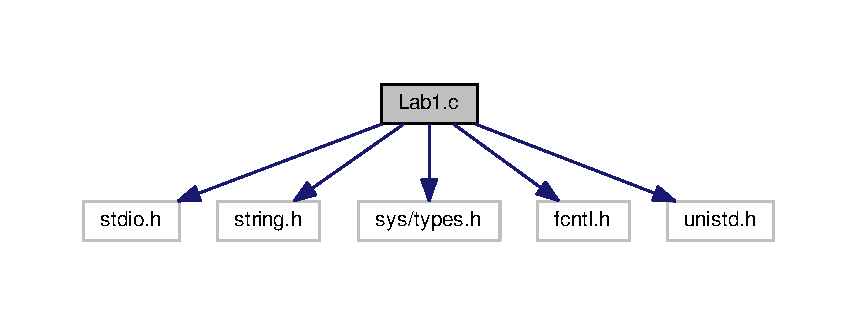
\includegraphics[width=350pt]{Lab1_8c__incl}
\end{center}
\end{figure}
\subsection*{Functions}
\begin{DoxyCompactItemize}
\item 
int \hyperlink{Lab1_8c_a0ddf1224851353fc92bfbff6f499fa97}{main} (int argc, char $\ast$argv\mbox{[}$\,$\mbox{]})
\end{DoxyCompactItemize}
\subsection*{Variables}
\begin{DoxyCompactItemize}
\item 
char \hyperlink{Lab1_8c_a1c03ec9f00c9255d336e34dbd17e89f2}{text} \mbox{[}1024\mbox{]}
\item 
char \hyperlink{Lab1_8c_a172e0aa8e5e6d24d62a8fa7e940d6d08}{dest\+\_\+loc} \mbox{[}128\mbox{]}
\item 
int \hyperlink{Lab1_8c_ae5163ff230abd4115d86194ad89467b5}{dest}
\item 
int \hyperlink{Lab1_8c_a07a87b2e6ed927503e2f95f119c9fc23}{source}
\item 
int \hyperlink{Lab1_8c_acab531abaa74a7e664e3986f2522b33a}{r}
\item 
int \hyperlink{Lab1_8c_aac374e320caaadeca4874add33b62af2}{w}
\end{DoxyCompactItemize}


\subsection{Function Documentation}
\index{Lab1.\+c@{Lab1.\+c}!main@{main}}
\index{main@{main}!Lab1.\+c@{Lab1.\+c}}
\subsubsection[{\texorpdfstring{main(int argc, char $\ast$argv[])}{main(int argc, char *argv[])}}]{\setlength{\rightskip}{0pt plus 5cm}int main (
\begin{DoxyParamCaption}
\item[{int}]{argc, }
\item[{char $\ast$}]{argv\mbox{[}$\,$\mbox{]}}
\end{DoxyParamCaption}
)}\hypertarget{Lab1_8c_a0ddf1224851353fc92bfbff6f499fa97}{}\label{Lab1_8c_a0ddf1224851353fc92bfbff6f499fa97}

\begin{DoxyCode}
11 \{
12    \textcolor{keywordflow}{if}(argc > 3)
13    \{
14       printf(\textcolor{stringliteral}{"ERROR: Usage %s <file name>\(\backslash\)n"}, argv[0]);
15       \_exit(1);
16    \}
17 
18    \hyperlink{Lab1_8c_a07a87b2e6ed927503e2f95f119c9fc23}{source} = 0;
19    \hyperlink{Lab1_8c_ae5163ff230abd4115d86194ad89467b5}{dest} = 0;
20 
21    \textcolor{keywordflow}{if}(argc == 3)
22    \{
23       printf(\textcolor{stringliteral}{"I will copy content of "});
24       printf(\textcolor{stringliteral}{"%s"}, argv[1]);
25       printf(\textcolor{stringliteral}{" to "});
26       printf(\textcolor{stringliteral}{"%s\(\backslash\)n"}, argv[2]);
27       \hyperlink{Lab1_8c_a07a87b2e6ed927503e2f95f119c9fc23}{source} = open(argv[1], O\_RDONLY);
28       \textcolor{keywordflow}{if}(\hyperlink{Lab1_8c_a07a87b2e6ed927503e2f95f119c9fc23}{source} == -1)
29       \{
30          printf(\textcolor{stringliteral}{"ERROR: %s does not exist\(\backslash\)n"}, argv[1]);
31          \_exit(1);
32       \}
33       strcpy(\hyperlink{Lab1_8c_a172e0aa8e5e6d24d62a8fa7e940d6d08}{dest\_loc}, argv[2]);
34    \}
35 
36    \textcolor{keywordflow}{if}(argc == 2)
37    \{
38       printf(\textcolor{stringliteral}{"I will save whatever you type into %s. Enter CTRL+D when done\(\backslash\)n"}, argv[1]);
39       strcpy(\hyperlink{Lab1_8c_a172e0aa8e5e6d24d62a8fa7e940d6d08}{dest\_loc}, argv[1]);
40    \}
41 
42    \textcolor{keywordflow}{if}(argc == 1)
43       printf(\textcolor{stringliteral}{"I will echo standard input to standard output! Enter CTRL+D when done\(\backslash\)n"});
44 
45    \textcolor{keywordflow}{if}(argc == 3 | argc == 2)
46    \{
47       \hyperlink{Lab1_8c_ae5163ff230abd4115d86194ad89467b5}{dest} = open(\hyperlink{Lab1_8c_a172e0aa8e5e6d24d62a8fa7e940d6d08}{dest\_loc}, O\_RDWR|O\_CREAT|O\_TRUNC, S\_IRUSR|S\_IWUSR|S\_IRGRP|S\_IWGRP);
48       \textcolor{keywordflow}{if}(\hyperlink{Lab1_8c_ae5163ff230abd4115d86194ad89467b5}{dest} == -1)
49       \{
50          printf(\textcolor{stringliteral}{"ERROR: %s could not open\(\backslash\)n"}, argv[2]);
51          \_exit(1);
52       \}
53    \}
54 
55    \textcolor{keywordflow}{do}
56    \{
57       \hyperlink{Lab1_8c_acab531abaa74a7e664e3986f2522b33a}{r} = read(\hyperlink{Lab1_8c_a07a87b2e6ed927503e2f95f119c9fc23}{source}, \hyperlink{Lab1_8c_a1c03ec9f00c9255d336e34dbd17e89f2}{text}, 1024);
58       \textcolor{keywordflow}{if}(\hyperlink{Lab1_8c_acab531abaa74a7e664e3986f2522b33a}{r} == -1)
59       \{
60          printf(\textcolor{stringliteral}{"ERROR: system could not read from terminal\(\backslash\)n"});
61          \_exit(1);
62       \}
63       \hyperlink{Lab1_8c_aac374e320caaadeca4874add33b62af2}{w} = write(\hyperlink{Lab1_8c_ae5163ff230abd4115d86194ad89467b5}{dest}, &\hyperlink{Lab1_8c_a1c03ec9f00c9255d336e34dbd17e89f2}{text}, \hyperlink{Lab1_8c_acab531abaa74a7e664e3986f2522b33a}{r});
64       \textcolor{keywordflow}{if}(\hyperlink{Lab1_8c_aac374e320caaadeca4874add33b62af2}{w} == -1)
65       \{
66          printf(\textcolor{stringliteral}{"ERROR: %s could not be written into\(\backslash\)n"}, argv[1]);
67          \_exit(1);
68       \}
69    \} \textcolor{keywordflow}{while}(\hyperlink{Lab1_8c_acab531abaa74a7e664e3986f2522b33a}{r} > 0);
70 
71    \textcolor{keywordflow}{if}(close(\hyperlink{Lab1_8c_a07a87b2e6ed927503e2f95f119c9fc23}{source}) == -1)
72    \{
73       printf(\textcolor{stringliteral}{"ERROR: system could not close terminal\(\backslash\)n"});
74       \_exit(1);
75    \}
76    \textcolor{keywordflow}{if}(argc == 2 | argc == 3)
77    \{
78       \textcolor{keywordflow}{if}(close(\hyperlink{Lab1_8c_ae5163ff230abd4115d86194ad89467b5}{dest}) == -1)
79       \{
80          printf(\textcolor{stringliteral}{"ERROR: %s could not close\(\backslash\)n"}, argv[1]);
81          \_exit(1);
82       \}
83    \}
84 
85    printf(\textcolor{stringliteral}{"done!\(\backslash\)n"});
86 
87    \textcolor{keywordflow}{return} 0;
88 \}
\end{DoxyCode}


\subsection{Variable Documentation}
\index{Lab1.\+c@{Lab1.\+c}!dest@{dest}}
\index{dest@{dest}!Lab1.\+c@{Lab1.\+c}}
\subsubsection[{\texorpdfstring{dest}{dest}}]{\setlength{\rightskip}{0pt plus 5cm}int dest}\hypertarget{Lab1_8c_ae5163ff230abd4115d86194ad89467b5}{}\label{Lab1_8c_ae5163ff230abd4115d86194ad89467b5}
\index{Lab1.\+c@{Lab1.\+c}!dest\+\_\+loc@{dest\+\_\+loc}}
\index{dest\+\_\+loc@{dest\+\_\+loc}!Lab1.\+c@{Lab1.\+c}}
\subsubsection[{\texorpdfstring{dest\+\_\+loc}{dest_loc}}]{\setlength{\rightskip}{0pt plus 5cm}char dest\+\_\+loc\mbox{[}128\mbox{]}}\hypertarget{Lab1_8c_a172e0aa8e5e6d24d62a8fa7e940d6d08}{}\label{Lab1_8c_a172e0aa8e5e6d24d62a8fa7e940d6d08}
\index{Lab1.\+c@{Lab1.\+c}!r@{r}}
\index{r@{r}!Lab1.\+c@{Lab1.\+c}}
\subsubsection[{\texorpdfstring{r}{r}}]{\setlength{\rightskip}{0pt plus 5cm}int r}\hypertarget{Lab1_8c_acab531abaa74a7e664e3986f2522b33a}{}\label{Lab1_8c_acab531abaa74a7e664e3986f2522b33a}
\index{Lab1.\+c@{Lab1.\+c}!source@{source}}
\index{source@{source}!Lab1.\+c@{Lab1.\+c}}
\subsubsection[{\texorpdfstring{source}{source}}]{\setlength{\rightskip}{0pt plus 5cm}int source}\hypertarget{Lab1_8c_a07a87b2e6ed927503e2f95f119c9fc23}{}\label{Lab1_8c_a07a87b2e6ed927503e2f95f119c9fc23}
\index{Lab1.\+c@{Lab1.\+c}!text@{text}}
\index{text@{text}!Lab1.\+c@{Lab1.\+c}}
\subsubsection[{\texorpdfstring{text}{text}}]{\setlength{\rightskip}{0pt plus 5cm}char text\mbox{[}1024\mbox{]}}\hypertarget{Lab1_8c_a1c03ec9f00c9255d336e34dbd17e89f2}{}\label{Lab1_8c_a1c03ec9f00c9255d336e34dbd17e89f2}
\index{Lab1.\+c@{Lab1.\+c}!w@{w}}
\index{w@{w}!Lab1.\+c@{Lab1.\+c}}
\subsubsection[{\texorpdfstring{w}{w}}]{\setlength{\rightskip}{0pt plus 5cm}int w}\hypertarget{Lab1_8c_aac374e320caaadeca4874add33b62af2}{}\label{Lab1_8c_aac374e320caaadeca4874add33b62af2}

%--- End generated contents ---

% Index
\backmatter
\newpage
\phantomsection
\clearemptydoublepage
\addcontentsline{toc}{chapter}{Index}
\printindex

\end{document}
